\documentclass[11pt,a4paper]{article}

\usepackage[T1]{fontenc}
\usepackage[utf8]{inputenc}
\usepackage{graphicx}
\usepackage{booktabs}
\usepackage{amsmath}
\usepackage{geometry}
\usepackage{siunitx}
\usepackage{caption}

\geometry{margin=2.4cm}
\captionsetup{font=small}
\sisetup{detect-all}

\title{RSS-Based Access Point Localization Experiment}
\author{}
\date{}

\begin{document}
\maketitle

\section{Experimental Setup}

This experiment evaluates RSS-based localization for a single Wi-Fi access point
inside the Faculty of Engineering at Ferdowsi University of Mashhad. The target
access point was located in a corridor area of the building. An independently
measured coordinate was kept only as ground truth for final error evaluation:

\begin{center}
\texttt{36 deg 18'46.1"N, 59 deg 31'34.9"E}
\end{center}

which corresponds to:

\begin{center}
\texttt{latitude = 36.3128055556,\quad longitude = 59.5263611111}.
\end{center}

The experiment uses the pivot RSS table as the only RSS data source:

\begin{center}
\texttt{data/pivot\_signal\_table.csv}
\end{center}

The floor map was obtained from:

\begin{center}
\texttt{data/map.json}
\end{center}

The room and corridor outlines were drawn from the \texttt{map\_space\_coordinate}
table in the map JSON file.

\section{Dataset Description}

Each row in the pivot table contains the measurement position and the RSS values
observed from multiple Wi-Fi access points. A value of \SI{-100}{dBm} was treated
as a missing or non-detected RSS observation. For the selected target access
point, the number of valid RSS samples was 1069.

The selected access point was:

\begin{center}
\texttt{BSSID = b28ba99a8d2a}
\end{center}

\begin{table}[h]
\centering
\caption{Summary of RSS samples for the selected access point.}
\label{tab:data-summary}
\begin{tabular}{lr}
\toprule
Quantity & Value \\
\midrule
Valid RSS samples & 1069 \\
Maximum RSS & \SI{-29.0}{dBm} \\
Mean RSS & \SI{-72.89}{dBm} \\
RSS-weighted centroid error from ground truth & \SI{1.37}{m} \\
\bottomrule
\end{tabular}
\end{table}

Figure~\ref{fig:rss-map} shows the RSS measurements of the selected access point
overlaid on the building map. Stronger RSS values are shown in green, while
weaker RSS values are shown in red.

\begin{figure}[h]
\centering
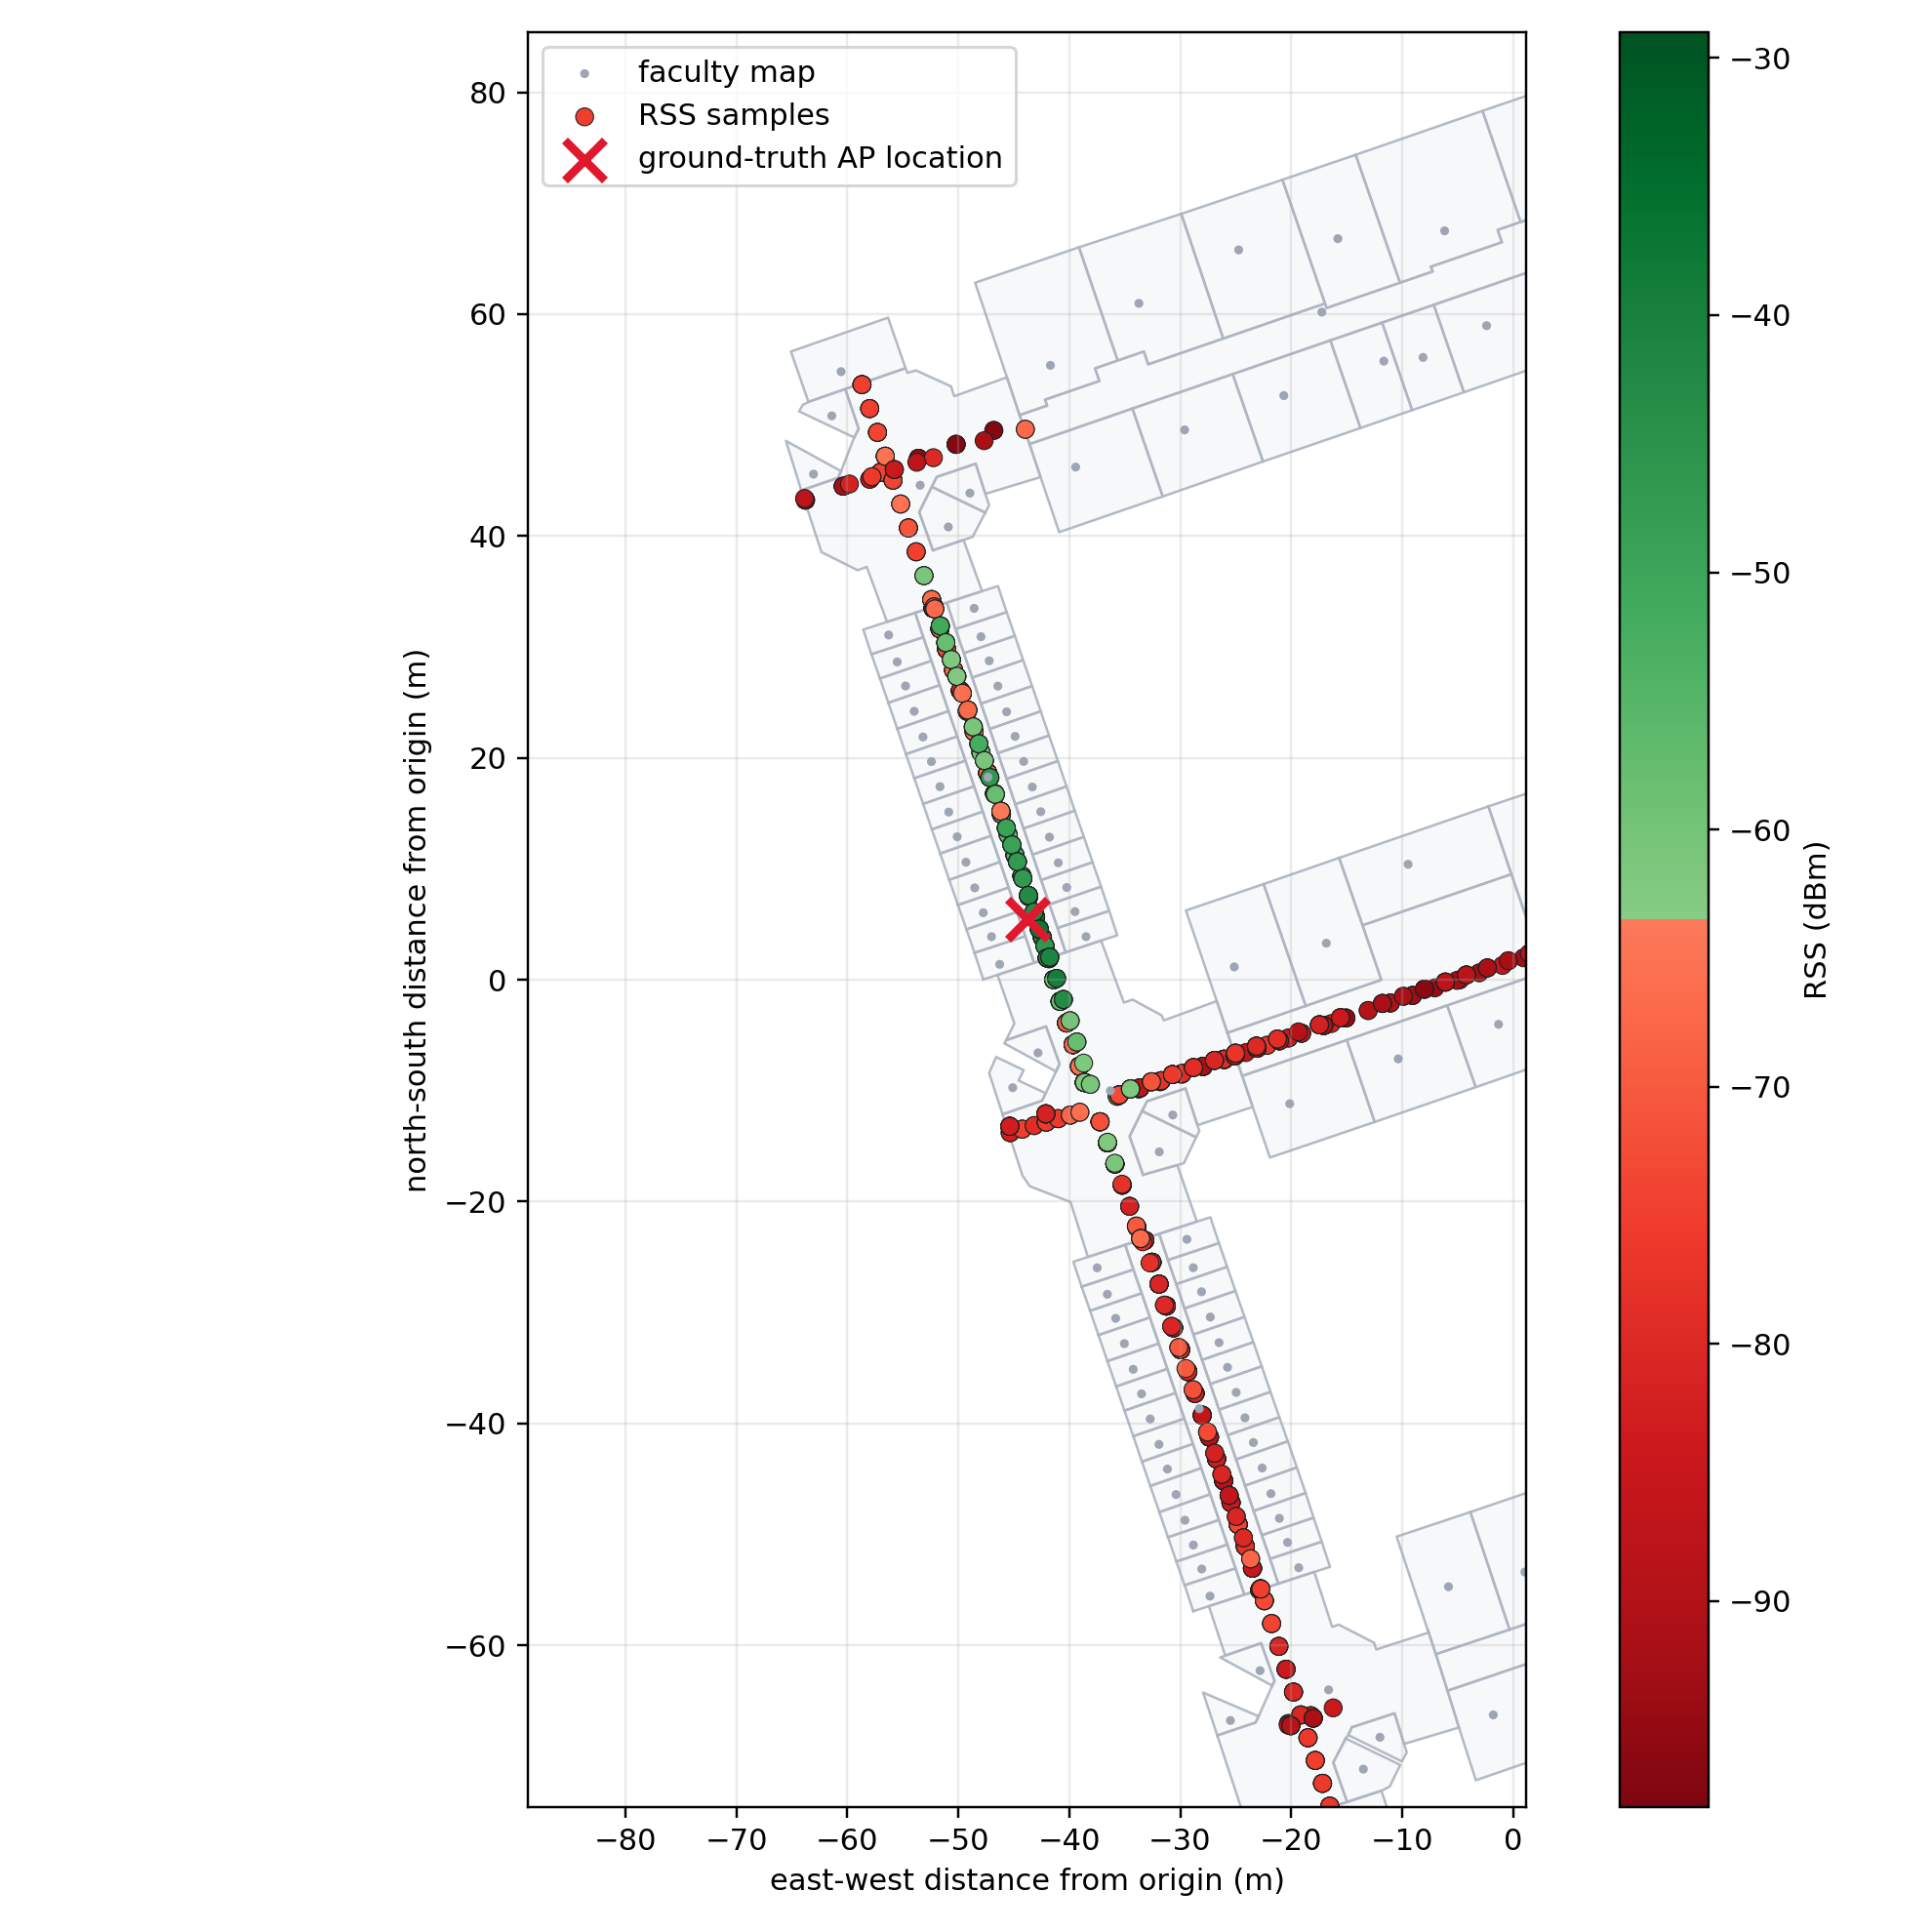
\includegraphics[width=0.92\textwidth]{figures/rss_map.png}
\caption{RSS samples of the selected access point overlaid on the faculty map.}
\label{fig:rss-map}
\end{figure}

\section{Access Point Selection}

To identify the access point corresponding to the target corridor location, all
RSS columns in the pivot table were examined. For each access point, only valid
RSS observations, i.e., samples with RSS greater than \SI{-100}{dBm}, were used.
An RSS-weighted spatial centroid was then computed for each candidate access
point.

For a sample with RSS value \(r_i\), the weight was defined as:

\begin{equation}
w_i = 10^{(r_i - r_{\max}) / 10},
\end{equation}

where \(r_{\max}\) is the strongest RSS observed for that access point. The
weighted centroid was computed as:

\begin{equation}
x_c = \frac{\sum_i w_i x_i}{\sum_i w_i},
\qquad
y_c = \frac{\sum_i w_i y_i}{\sum_i w_i}.
\end{equation}

The selected access point was \texttt{b28ba99a8d2a}. The ground-truth coordinate
was not used as an optimization input; it was used only to report the final
localization error.

\section{RSS Fitting Model}

After selecting the target access point, its location was estimated by fitting a
log-distance path-loss model to the RSS measurements. The model is:

\begin{equation}
RSS(d) = RSS_{1m} - 10n\log_{10}(d),
\end{equation}

where \(RSS_{1m}\) is the estimated RSS at one meter, \(n\) is the path-loss
exponent, and \(d\) is the Euclidean distance between a measurement location and
the estimated access point position.

The fitted parameter vector was:

\begin{equation}
\theta = (x_{AP}, y_{AP}, RSS_{1m}, n).
\end{equation}

For measurement point \(i\), with local Cartesian coordinate \((x_i,y_i)\), the
distance to a candidate AP position is:

\begin{equation}
d_i(\theta)=\max\left(\sqrt{(x_i-x_{AP})^2+(y_i-y_{AP})^2}, 1\right).
\end{equation}

The lower bound of \SI{1}{m} prevents numerical instability in the logarithmic
model when the candidate AP position becomes very close to a measurement point.
The predicted RSS is:

\begin{equation}
\widehat{r}_i(\theta)=RSS_{1m}-10n\log_{10}\left(d_i(\theta)\right),
\end{equation}

and the residual is:

\begin{equation}
e_i(\theta)=\widehat{r}_i(\theta)-r_i,
\end{equation}

where \(r_i\) is the measured RSS. The parameters were estimated by solving the
following robust nonlinear least-squares problem:

\begin{equation}
\min_{\theta}\; \frac{1}{2}\sum_{i=1}^{N}\rho\left(e_i(\theta)^2\right).
\end{equation}

The selected robust loss was the \texttt{soft\_l1} loss:

\begin{equation}
\rho(z)=2\left(\sqrt{1+z}-1\right).
\end{equation}

This loss is close to the ordinary squared loss for small residuals, but grows
more slowly for large residuals. Therefore, strong RSS outliers have less effect
on the fitted AP location, which is important in indoor environments with
multipath propagation, shadowing, and device-orientation effects.

The fitting procedure was performed step by step as follows:

\begin{enumerate}
\item Measurement coordinates were first converted from latitude and longitude
to a local Cartesian coordinate system in meters.

\item The valid RSS samples of the selected AP were retained, and missing
detections were excluded.

\item The initial AP position was set to the measurement point with the maximum
RSS value. Therefore, the ground-truth coordinate was not used to initialize the
optimization.

\item The initial \(RSS_{1m}\) value was set from a high RSS percentile, and the
initial path-loss exponent was set to \(n=2\).

\item Bound constraints were applied during optimization. The AP coordinates
were allowed to move within the observed measurement region with an additional
margin, \(RSS_{1m}\) was constrained to a realistic RSS range, and the path-loss
exponent was constrained to \(0.5 \le n \le 6\).

\item For each candidate AP position and model parameter set, distances from the
candidate AP to all measurement points were computed, and RSS values were
predicted using the log-distance model.

\item The optimizer evaluated the residual vector, applied the robust loss, and
iteratively updated \((x_{AP},y_{AP},RSS_{1m},n)\) until the objective function
no longer changed significantly.

\item After convergence, the estimated AP position was converted back to
latitude and longitude. The ground-truth coordinate was used only at this final
stage to compute localization error.
\end{enumerate}

\section{Localization Results}

Table~\ref{tab:fit-result} summarizes the localization and model-fitting
results.

\begin{table}[h]
\centering
\caption{Estimated AP location and fitted RSS model parameters.}
\label{tab:fit-result}
\begin{tabular}{lr}
\toprule
Quantity & Value \\
\midrule
Initial latitude & 36.3127978000 \\
Initial longitude & 59.5263734000 \\
Estimated latitude & 36.3128106176 \\
Estimated longitude & 59.5263414105 \\
Distance from ground truth & \SI{1.85}{m} \\
Estimated \(RSS_{1m}\) & \SI{-28.36}{dBm} \\
Path-loss exponent \(n\) & 3.22 \\
RSS RMSE & \SI{8.53}{dB} \\
RSS MAE & \SI{6.91}{dB} \\
\bottomrule
\end{tabular}
\end{table}

Figure~\ref{fig:estimated-map} shows the ground-truth AP coordinate and the
estimated AP position on the building map. The red cross indicates the
ground-truth coordinate, and the black star indicates the estimated AP location.

\begin{figure}[h]
\centering
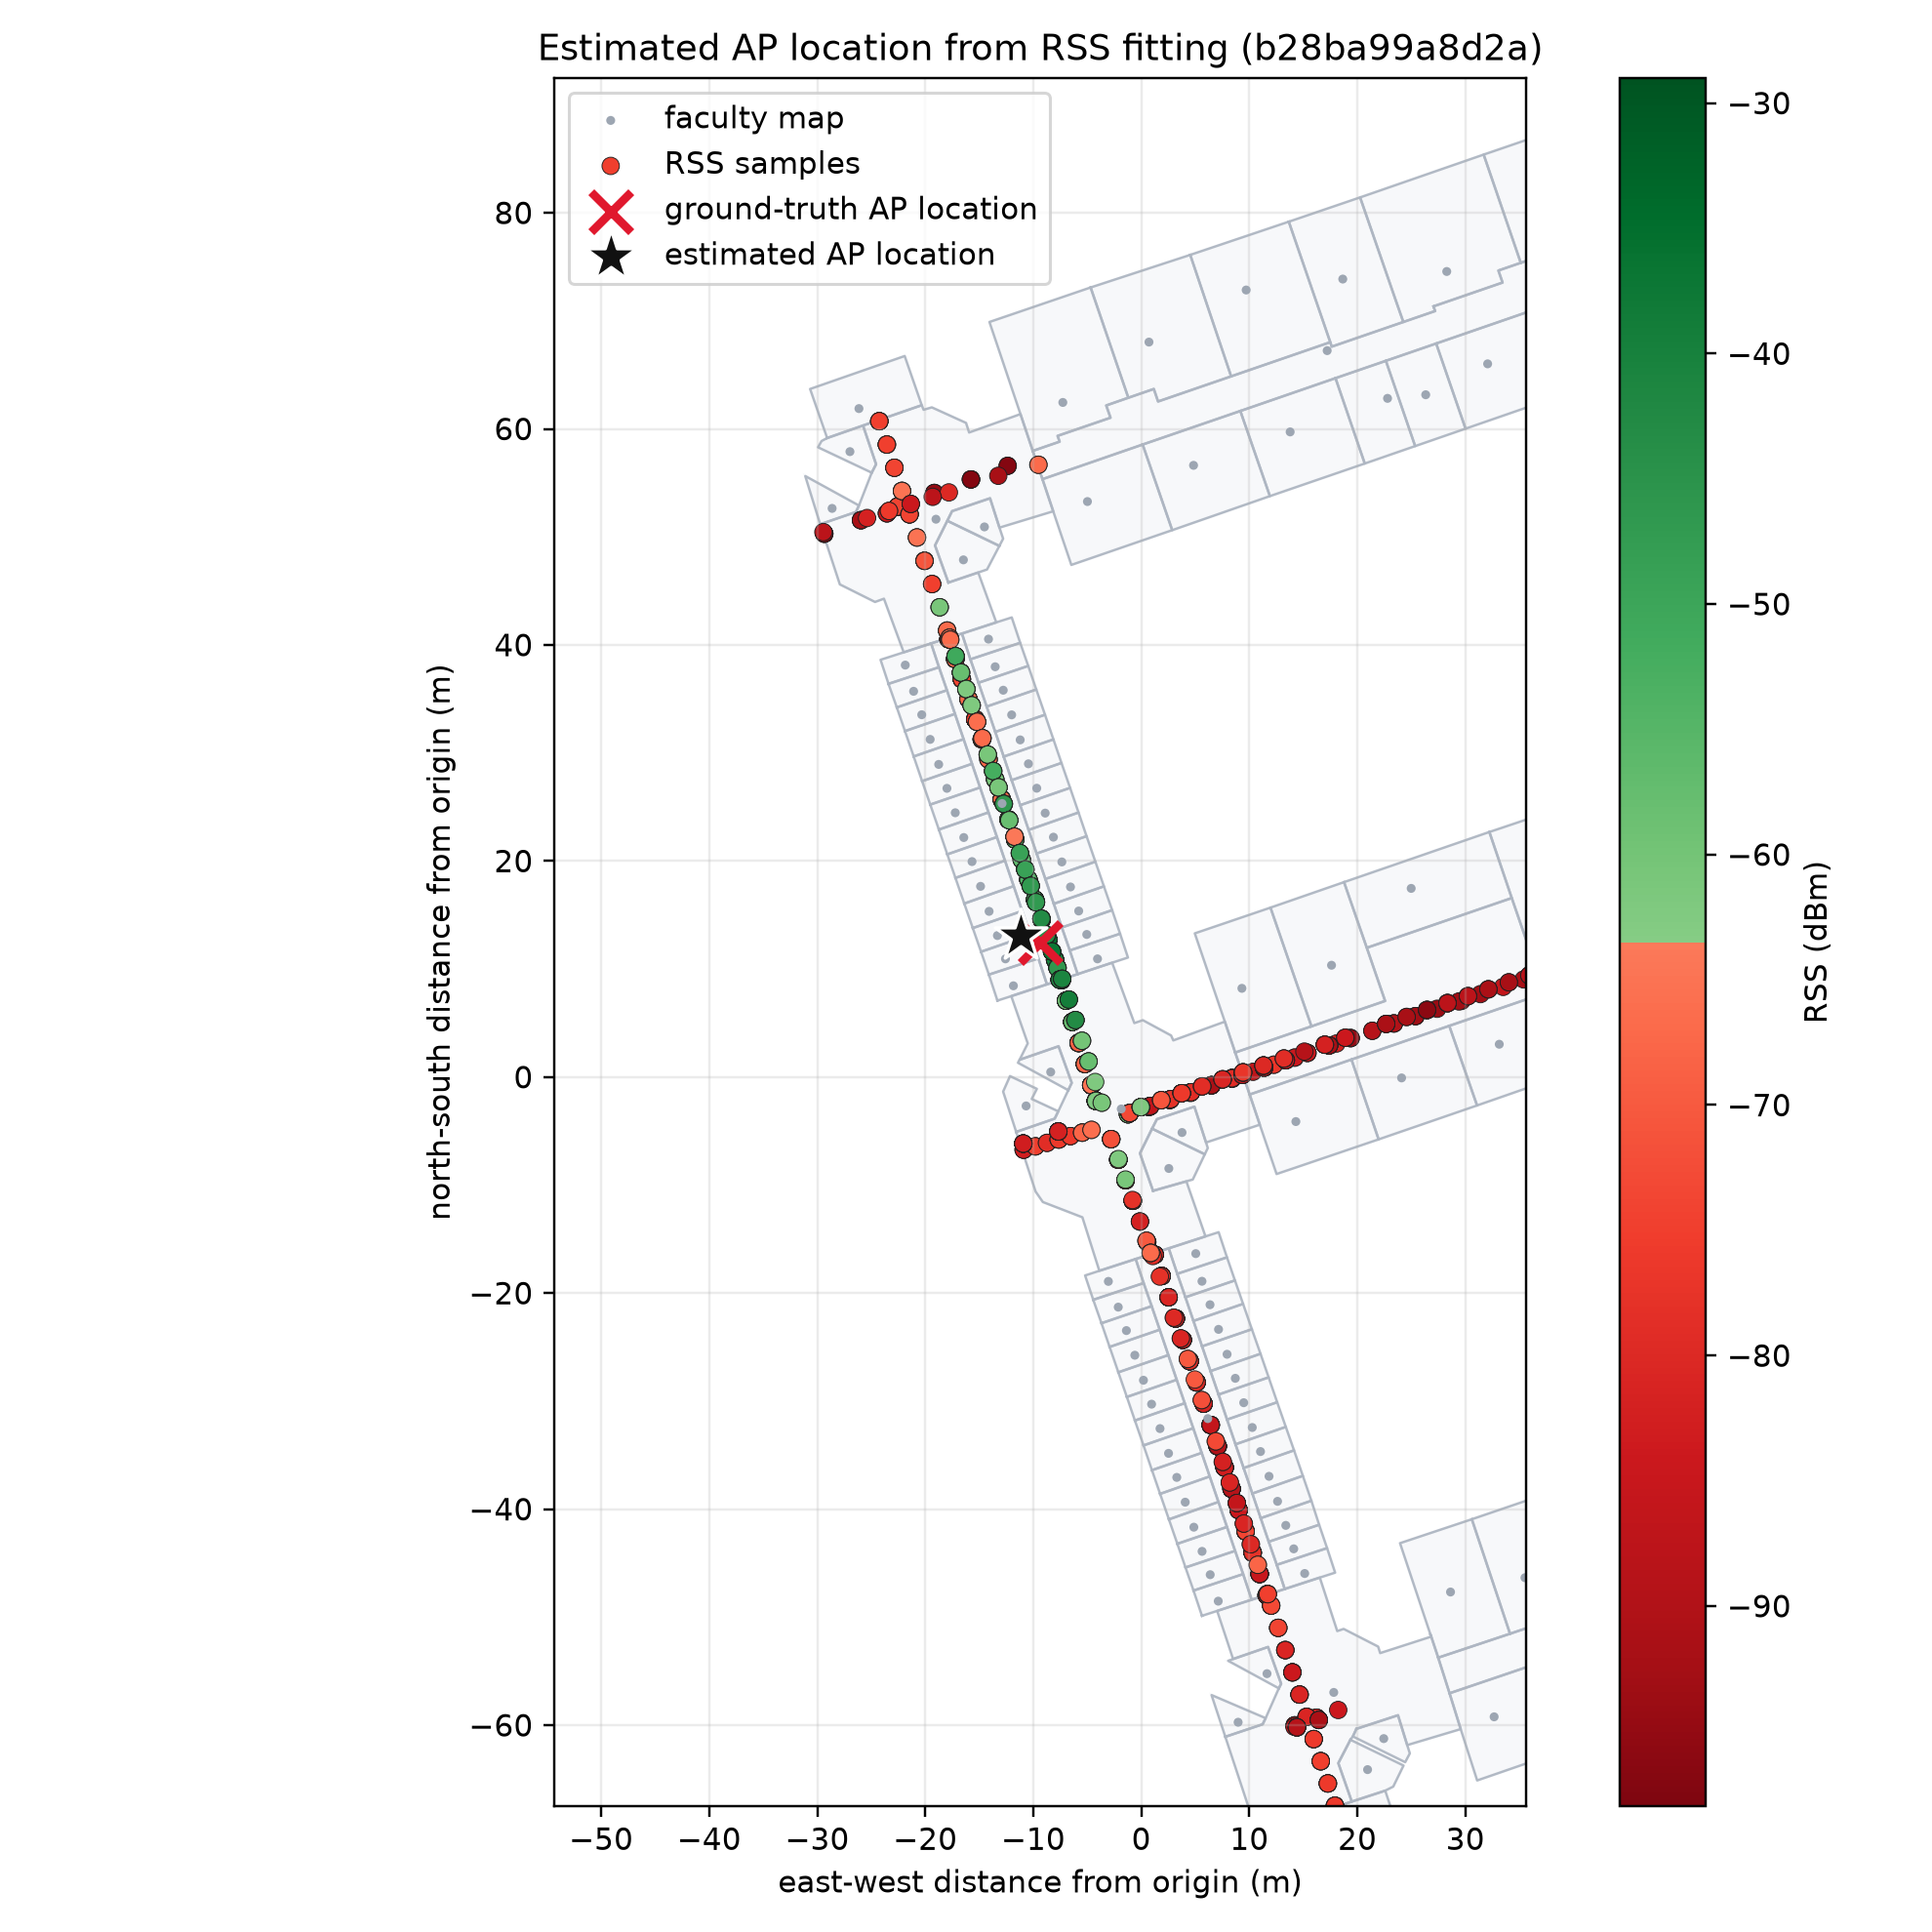
\includegraphics[width=0.92\textwidth]{figures/estimated_ap_map.png}
\caption{Reference and estimated access point locations on the faculty map.}
\label{fig:estimated-map}
\end{figure}

The estimated position was approximately \SI{1.85}{m} away from the ground-truth
coordinate. Considering the high variability of indoor RSS measurements, this
result indicates that the fitted log-distance model can provide a practical
approximation of the access point location when sufficient RSS samples are
available around the target area.

\end{document}
